\chapter{Project Scope Management}

The Tennis Club Web Service (TCWS) project will provide clients and customers with the features that they need in the daily running of the club. As we are dealing with personal information of club members including billing data, security is one of the main non-functional requirements (or quality requirements as Lauesen titled them) of the web site. The project will use Spring Framework, Hibernate, Tomcat and Apache tiles to provide the service.
Scope will be validated with the relevant stakeholders when each module and milestone is completed.

Once a scope management plan is defined we can create a WBS for the project. We can also define how formal acceptance of complete project tasks can be verified.

\section{Plan Scope Management}

In this phase of the project we will create a scope management plan and a requirements management plan. The scope management plan is a component of the project or program management plan that describes how the scope will be defined, developed, monitored, controlled, and verified \parencite{pmbok}. One the project charter is defined and analysed we can begin to develop the scope management plan.

Firstly project scope will be defined with a scope management plan which is defined at project initiation. Project scope will then be controlled by project managers in meetings with development teams, where the scope will be clearly outlined to employees. Meetings with management will be arranged weekly to monitor and control scope of the project. Development leads will meet with team members daily at stand-up meetings at the end of each day. Development leads will then report to middle management at weekly update meetings to update them on development progress. Any changes to the scope of the project will be outlined in these meetings to development leads so they can adjust plans accordingly.

\begin{enumerate}
\item The project manager will create a WBS from the project scope statement and will be the person in charge of maintaining and approving the scope.
\item The project manager, requirements analyst and development leads will formally approve and accept completed project deliverables. 
\item Requests for change to the project scope statement must be made formally to the project manager.
\end{enumerate}

Secondly a requirements management plan will be created to define how requirements will be analysed, documented and managed \parencite{pmbok}. We have decided that a hands-on relationship with the stakeholders and customers is the best way to collect requirements and the most effective way to find out if requirements change.


\begin{enumerate}
\item Requirements will be planned, tracked and reported through the requirements analyst, who confers with the project manager to decide if a requirement is included or excluded in scope. Or even part of future scope
\item The customer will be questioned on which requirements are the most important to them
\item Requirements will be traced using Atlassian Jira. This gives the requirements full traceability.
\end{enumerate}


\section{Collect Requirements}

The output from planning scope is a requirements management plan. This plan describes how requirements will be analysed documented and managed.
Requirements Elicitation is an important step in the development of a software application. There are a number of techniques possible, such as “interviewing, protocol analysis, repertory grid, work groups" \parencite{req}. 

Structured interviews “appear to be one of the most effective elicitation techniques in a wide range of domains and situations” \parencite{req}.
“The hardest part of building a software system is deciding what to build No other part of the work so cripples the resulting system if done wrong. No other part is more difficult to rectify later.” \parencite{brooks}.

In eliciting possible requirements for the site, there was a discussion with three club members with varying backgrounds and experience within the club.

At an early stage of the project, rough storyboards were prepared. These storyboards were used to demonstrate how a page, such as the timetable shown in Figure~\ref{fig:timetableSB}, would be displayed by the application. 

\begin{figure}[H]
\begin{center}
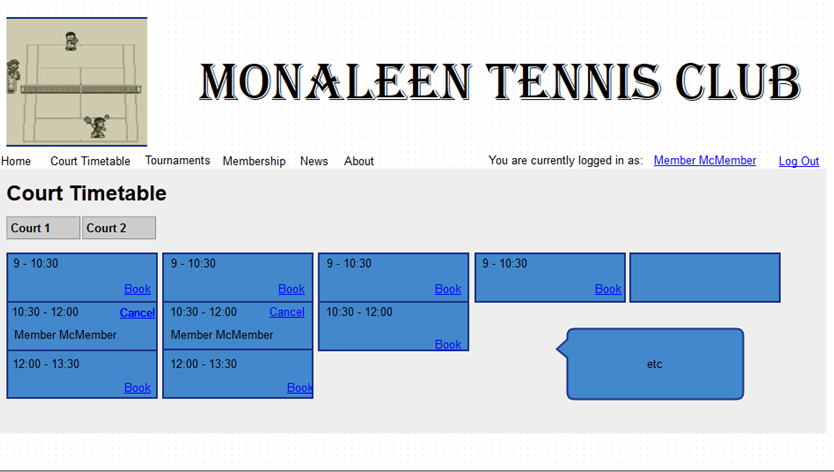
\includegraphics[width=14cm]{storyboard.png}
\end{center}
\caption{Timetable Storyboard, October 2013}
\label{fig:timetableSB}
\end{figure}

The storyboarding visualised aspects of the site, and gave a rough idea of functionality that would be needed within the application. These were shown to interviewees in order to help them visualise requirements.

The style of the timetable was based on the existing paper based solution currently implemented by the club, displayed in Figure~\ref{fig:papertt}.

\begin{figure}[H]
\begin{center}
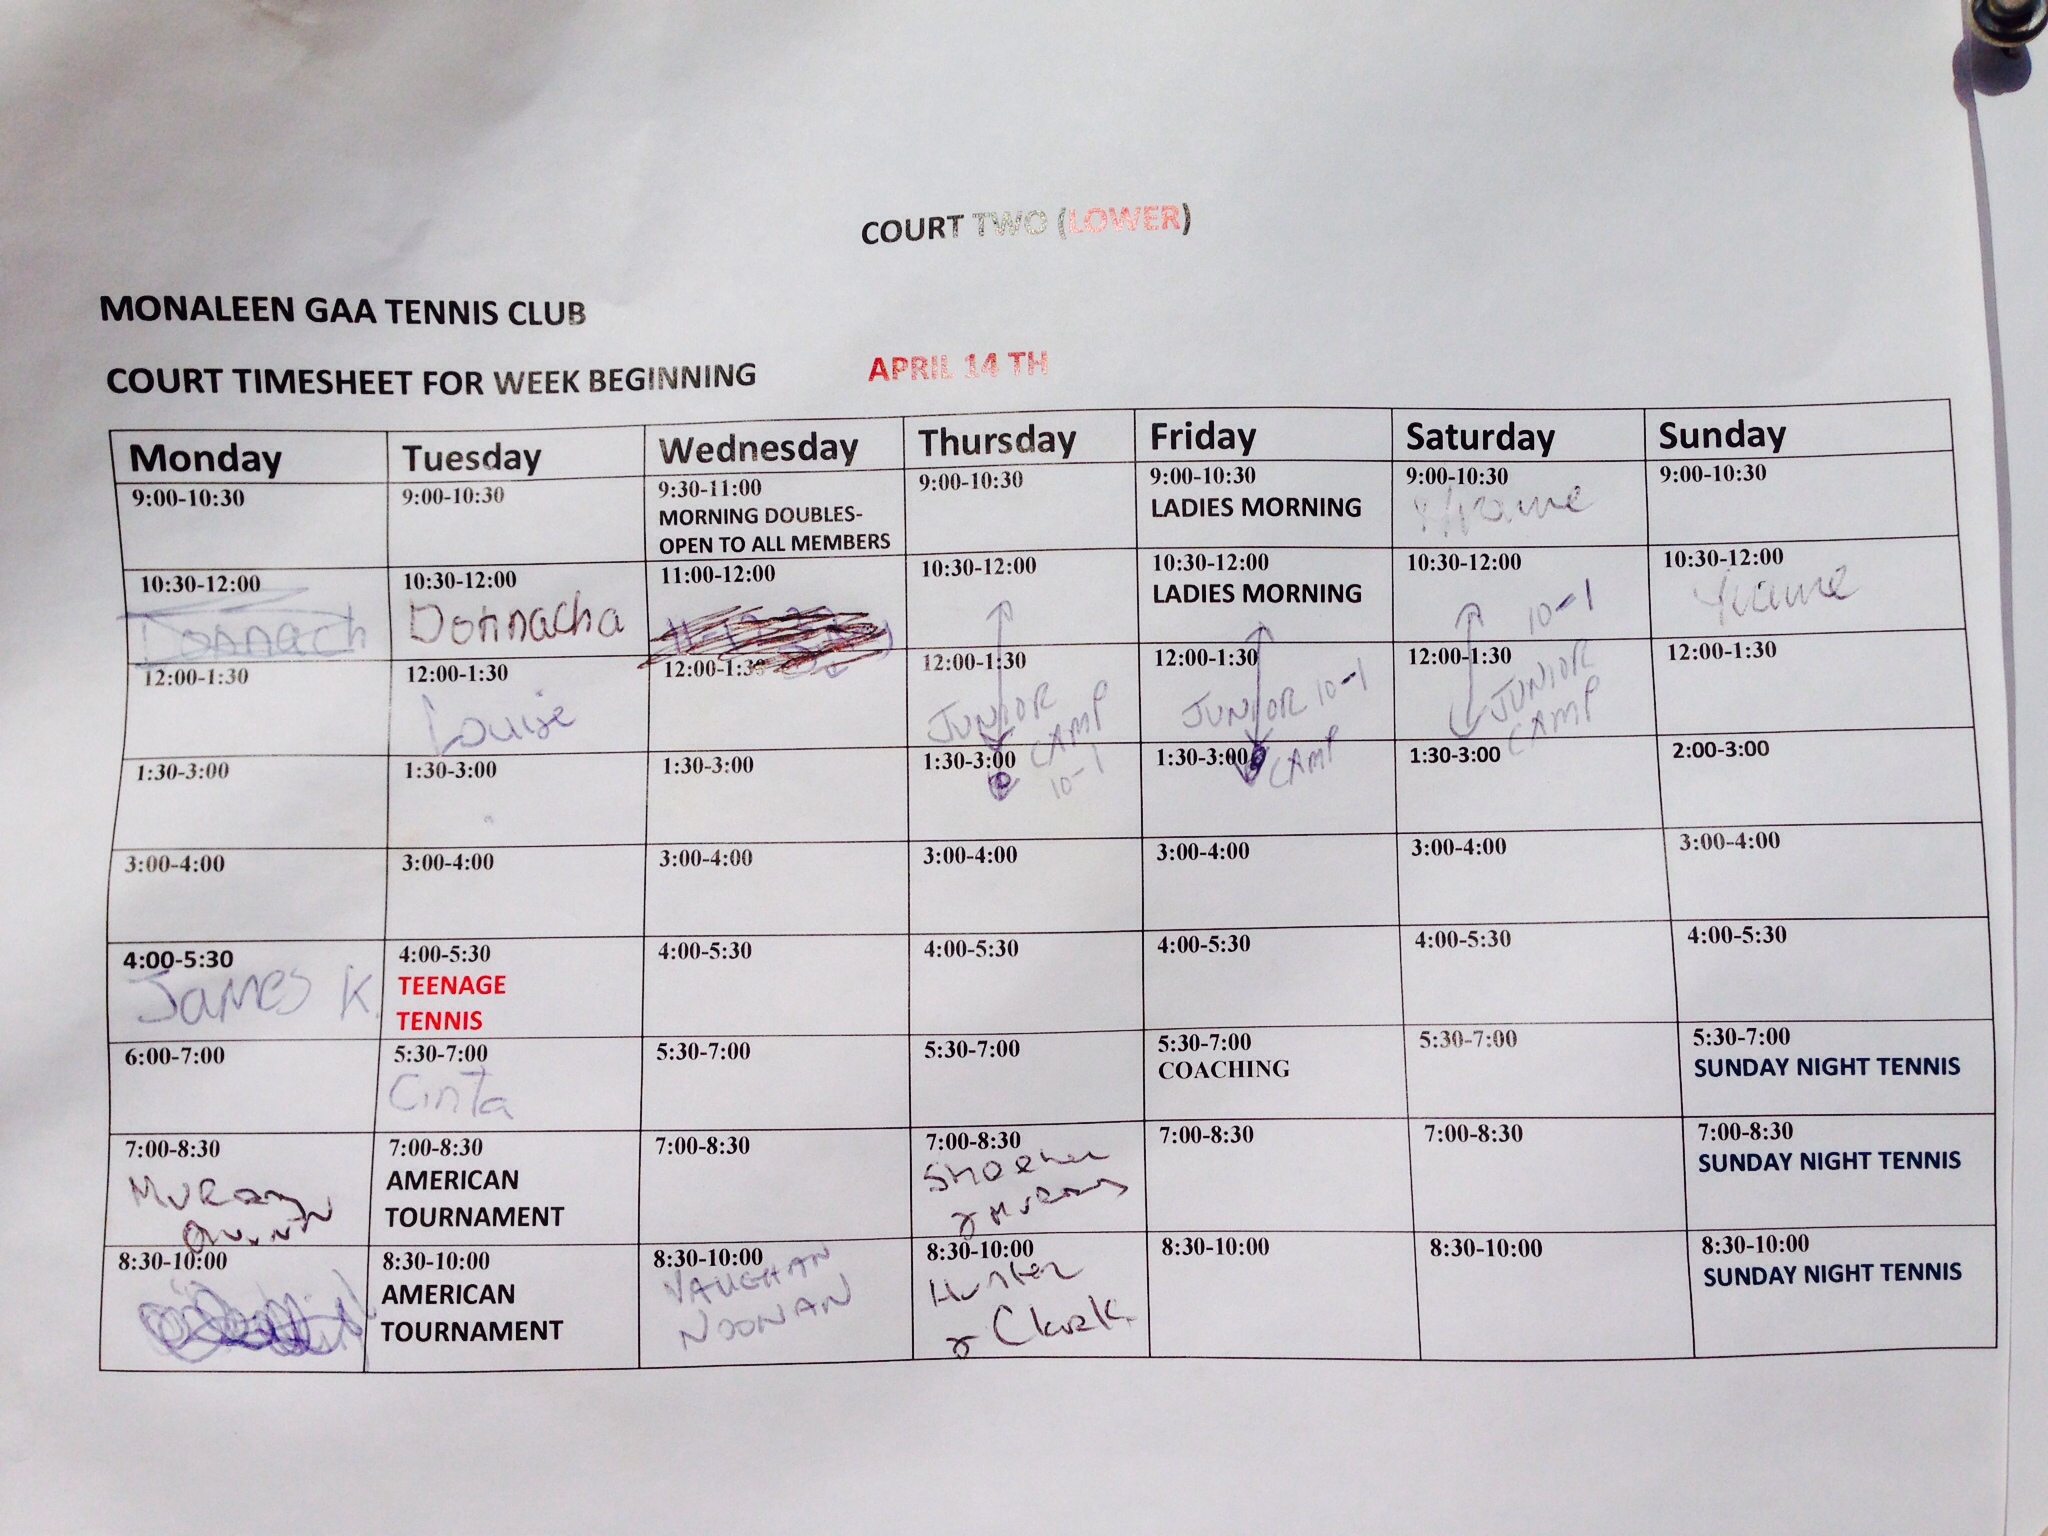
\includegraphics[width=14cm]{originaltt.jpg}
\end{center}
\caption{Paper Timetable, Monaleen Tennis Club}
\label{fig:papertt}
\end{figure}

\begin{table}[H]
\caption{Stakeholders for Requirements Elicitation}
\begin{center}
    \begin{tabular}{ | l | l | l | l | l| p{5cm} |}
    \hline
    Name & Age Bracket & Club Role & Club Membership & Work Background \\ \hline
	S1 & 35 - 45& Committee Member & 5 years & Senior Software Engineer \\ \hline
	S2 & 18 - 25 & New Member & 1 year & Graduate Software Engineer \\ \hline
	S3 & 55+ & Senior Member & 10+ years & Retired Public Servant \\ \hline
    \end{tabular}
\end{center}
\label{fig:userelicit}
\end{table}

In order to elicit requirements, a number of interviews were held with stakeholders. A set of questions were prepared as a guideline, and some storyboards were presented. The Tralee Tennis Club website was also presented to the interviewees:

\begin{enumerate}
\item Are you aware there is a site for Monaleen Tennis Club?
\item If are, what do you you it for?
\item What are the best features of the site? 
\item What features are needed?
\item If you were not aware, why? 
\item Would you use a website if you had known it was there?
\item Looking at the examples provided, are there any things you feel this club could benefit from?
\item How do you feel current tournaments are organised?
\item Is it easy to register for tournaments?
\item Have you ever had issues finding information about club events?
\item Do you know when club events are happening?
\item Is it easy to contact club members or find out how to contact them?
\item How easy is it to become a member/renew your membership?
\item How do you contact club committee members?  
\end{enumerate}


During the elicitation process a number of areas were highlight as desired features.

\begin{enumerate}
\item Online Timetable
\begin{itemize}
\item Allow members to view courts and make/view bookings
\end{itemize}
\item Tournaments
\begin{itemize}
\item Allow user to register for a tournament, and view tournaments ongoing.
\end{itemize}
\item Contact Members
\begin{itemize}
\item Easy way to contact all members
\end{itemize}
\item Member Directory
\begin{itemize}
\item A list of all members, contact details, roles
\end{itemize}
\item News Section
\begin{itemize}
\item Create new items to display for members
\end{itemize}
\item Members Area
\begin{itemize}
\item A secure area that only members could access
\end{itemize}
\item Member Application
\begin{itemize}
\item Automated registration, replace old paper form
\end{itemize}
\item Club Map
\begin{itemize}
\item Directions to the club for new members and non-local visitors
\end{itemize}
\item Contact Details
\begin{itemize}
\item Information on how to contact within the club for specific needs
\end{itemize}
\item Statistics
\begin{itemize}
\item Such as games played, Win/Loss ratio
\end{itemize}
\end{enumerate}
\begin{table}[H]
\label{fig:requirementsFeatures}
\caption{Requested Features}
\end{table}
Table ~\ref{fig:reqbreakdown} refers to each numbered requirement, and whether it was brought up by a stakeholder during the elicitation process.
\begin{table}[H]
\caption{Requested Feature Breakdown}
\begin{center}
    \begin{tabular}{ | l | l | l | l| l| l| l| l| l|l| p{.22cm} |}
    \hline
     \textit{Name}& 1& 2 & 3 & 4 & 5 & 6 & 7 & 8 & 9 & 10\\ \hline
	 S1 & N & Y & Y & Y & Y & Y & Y & Y & Y & N\\ \hline
	 S2 & Y & Y & Y & N & N & N & N & N & N & Y\\ \hline
	 S3 & Y & N & N & N & N & N & Y & Y & N & N\\ \hline
  Total & 2 & 2 & 2 & 1 & 1 & 1 & 2 & 2 & 1 & 1\\ \hline
    \end{tabular}
\end{center}
\label{fig:reqbreakdown}
\end{table}


\section{Scope Definition}

This section documents the scope of the tennis club website, i.e. what is included and excluded in the scope of the project.
Inputs:
\begin{enumerate}
\item Scope management plan
\item Project charter
\item Requirements documentation
\item Organisational process assets
\end{enumerate}

Outputs:
\begin{enumerate}
\item Project scope statement
\item Project documents updates
\end{enumerate}
\subsection{Included in Scope}

The following is an outline of what is included in the project management scope. A major goal of this project is to develop a general tennis club platform that can be applied to many clubs to maximise profit.

Functional Requirements:
\begin{enumerate}
\item Timetable for booking courts
\begin{itemize}
\item Flexible
\item Book slot
\item Unbook slot
\item Define a template for timetable (Admin)
\item Reset timetable (Admin)
\item Delete timetable (Admin)
\item Enable and disable timetable
\item Different clubs use different booking systems
\item Timetable Analysis
\end{itemize}

\item The tournament system is used by both players and administrators
\begin{itemize}
\item Players register an interest in a tournament
\item Admins use system to organise players into teams/matches
\item Create tournament
\item Delete tournament
\item Display tournament fixtures
\item Create singles/doubles/round-robin tournaments
\item Contact users registered for the tournament
\item Display tournament results
\item Register a result of a match (both players have to agree)
\end{itemize}
\item News Blog
\begin{itemize}
\item Create new post
\item Upload images
\item Rich text formatting
\item Embed videos from third party
\item Delete post
\item Edit post
\item Display Post
\end{itemize}
\item Members Services
\begin{itemize}
\item Registration
\item Members only access
\item Approve/Block members (Admin)
\item Delete expired members (Admin)
\item Contact all members (Admin)
\item View member list (Admin)
\item Pay membership fee
\item Buy equipment
\end{itemize}
\end{enumerate}

Also included in the scope of the project is a customer deployment team who can liaise with the customers to deploy the application either on cloud services or the customers dedicated servers.
Non-functional requirements (NFR) included in the scope are usability, security and extensibility.

To support the security NFR, user data must be securely sored in our databases. We are building a payment platform for members to pay their fees therefore we need to protect user billing data with the latest security standards. The company can come under legal scrutiny unless user data is handled appropriately.

We plan to support extensibility as a main NFR so that we can deal with changes to existing clubs and supporting different types of clubs with differing requirements. The main customer has two courts for users to book a slot in. The club has plans to expand in the future resulting in the creation of four new courts. The number of courts available for booking therefore needs to be dynamic. Often clubs use different types of tournaments, i.e. there is no one-size-fits-all tournament type that all clubs use. Our application needs to support ladder, bracket and league tournaments. The club also hosts tournaments with outside clubs; the ability to add non-members as a guest to our tournament system is required.

We are developing the system for a singular customer, however, there is room in the scope of the project to build a general platform that can be customised for each customer with minimal effort on the customer side. Simple settings like number of courts, type of tournaments and different payment plans are examples of features that could be provided.

The age of the club members range from 8 to 80, meaning ease of use of any software solution is important. If a system is going to replace the existing paper based system, a similar level of usability is required so all players can use it. The most common function used by members is the reservation of time slot for a court. A software alternative needs to be intuitive for all members.

\subsubsection{Excluded from Scope}

Excluded from the scope of the project is a social network for tennis players of the club. We researched what other solutions offered and while this type of feature would be cutting edge technology for our solution, it is not a feature that users are desperate for or requesting right now.

\subsubsection{Constraints}

The project has a tight budget and a low staff head count. The first customer also wants the product to be shipped in 6 months. Further, to justify adding multi club support to the product we need to find a second customer in the first 12 months of release; as this is a global product, this constraint should be low risk.

\section{Create WBS}

Creating the WBS is the process of subdividing project deliverables or work into smaller components

\begin{figure} [H]
\begin{center}
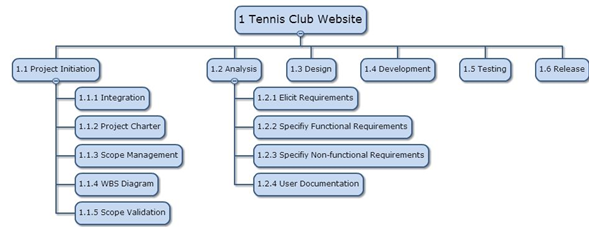
\includegraphics[scale=0.9]{wbs.png}
\caption{Work Breakdown Structure}
\label{fig:in1}
\end{center}
\end{figure}


\begin{figure} [H]
\begin{center}
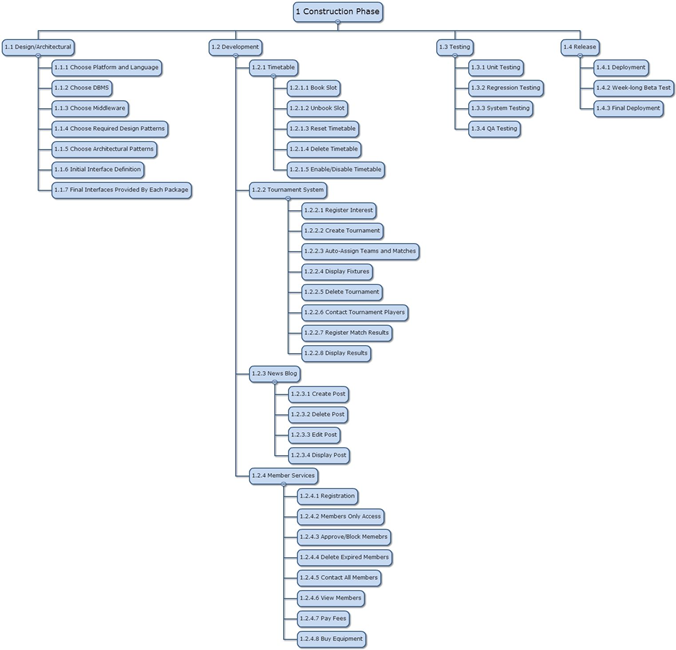
\includegraphics[scale=.9]{wbsbig.png}
\caption{Work Breakdown Structure - Construction Phase}
\label{fig:in1}
\end{center}
\end{figure}

\section{Validate Scope}

Validating scope is the process of formalizing acceptance of the completed project deliverables.

Validation can be achieved using two techniques: inspection and group decision making techniques. Inspections can be carried out using meeting styles like reviews, audits and walkthroughs. Audits can be executed in a group or individual setting. Walkthroughs are group activities only. Group decision techniques will also be used in this project. As this is a high stakes project, development leads, project managers, test team leads, customers and any other relevant stakeholders will be present at group meetings. The method we will use for reaching group decisions is a majority decision, as this is the fairest to all stakeholders. Group meetings will be held monthly.

\subsection{Outputs}

\subsubsection{Accepted Deliverables}

The accepted deliverables of this project are the following:
\begin{enumerate}
\item Timetable for booking courts
\item Tournament system to be used by both players and administrators
\item News Blog
\item Members Services
\end{enumerate}

These deliverables have been signed off on the by the project manager and the customer.

\section{Control Scope}

Controlling scope is the process of monitoring the status of the project and product scope. It also involves managing changes to the scope baselines and allows the scope baseline to be maintained throughout the project \parencite{pmbok}.

Variance analysis is the technique used to measure the difference between the baseline and actual project performance. This type of analysis also measures the cause of the variation. Using this technique we can determine whether we need to change the scope of the project. Variance analysis will be executed bi-weekly.
